% Revision summary (2026-04-07):
% - Reworked the document into an FYP-compliant dissertation package with title page,
%   abstract metadata, acknowledgements, table of contents, references before appendices,
%   and roman-to-arabic page numbering.
% - Reframed the thesis around the core empirical insight that statistical leadership and
%   economic signal leadership diverge in intraday IV-curve forecasting.
% - Strengthened the introduction, critical literature review, methodology, results
%   interpretation, and discussion so the document reads as one coherent study rather than
%   a stitched benchmark log.
% - Integrated the completed winner-versus-all-baselines appendix and block-bootstrap
%   significance analysis for the final retuned xLSTM benchmark.
% - Moved implementation architecture into the experimental-design chapter and added
%   appendices for dataset schema, benchmark configuration, and robustness notes.
% TODO metadata placeholders retained only where the source did not provide them:
% Project No, Advisor, Deliverables wording.
\documentclass[12pt]{report}

\usepackage[a4paper,margin=1in]{geometry}
\usepackage[T1]{fontenc}
\usepackage[utf8]{inputenc}
\usepackage{lmodern}
\usepackage{microtype}
\usepackage{setspace}
\usepackage{amsmath,amssymb}
\usepackage{booktabs}
\usepackage{array}
\usepackage{tabularx}
\usepackage{ragged2e}
\usepackage{graphicx}
\usepackage{float}
\usepackage{caption}
\usepackage{enumitem}
\usepackage{xcolor}
\usepackage{hyperref}
\usepackage{xurl}
\usepackage{tikz}
\usepackage[numbers]{natbib}

\usetikzlibrary{arrows.meta,positioning}
\hypersetup{colorlinks=true,linkcolor=blue,citecolor=blue,urlcolor=blue}
\renewcommand{\bibname}{References}
\setlength{\parindent}{0pt}
\setlength{\parskip}{0.55em}
\setlength{\emergencystretch}{2em}
\onehalfspacing
\captionsetup{font=small}
\newcolumntype{Y}{>{\RaggedRight\arraybackslash}X}
\newcommand{\assetroot}{thesis_report_assets}
\newcommand{\code}[1]{\begingroup\ttfamily\path{#1}\endgroup}
\newcommand{\insertassetfigure}[3]{%
\begin{figure}[H]
\centering
\IfFileExists{\assetroot/figures/#3}{\includegraphics[width=0.92\textwidth]{\assetroot/figures/#3}}{\fbox{\parbox[c][2.2in][c]{0.85\textwidth}{\centering Missing figure}}}
\caption{#1}
\label{#2}
\end{figure}}

\begin{document}
\hypersetup{pageanchor=false}

\begin{titlepage}
\thispagestyle{empty}
\centering

{\Large B.Comp. Dissertation\par}
\vspace{1.0cm}

{\Huge\bfseries Intraday Options Mispricing Detection via Implied-Volatility Curve Forecasting
}
\vspace{1.4cm}

{\Large James Shen\par}
\vspace{0.5cm}
{\large School of Computing, National University of Singapore\par}
\vspace{1.0cm}

\begin{tabular}{@{}ll@{}}
Academic Year: & 2025/2026 \\
Project No: & TODO \\
Advisor: & Prof. Lu Yao \\
\end{tabular}

\vfill

\begin{minipage}{0.82\textwidth}
\textbf{Deliverables}
\begin{itemize}[leftmargin=1.2cm,itemsep=0.15em]
    \item Dissertation report and appendices.
    \item Reproducible Python codebase for data processing, model training, and evaluation.
    \item Thesis asset pack containing figures, tables, and supporting experiment summaries.
\end{itemize}
\end{minipage}

\vfill
{\large April 2026\par}
\end{titlepage}

\cleardoublepage
\setcounter{page}{1}
\pagenumbering{roman}

\chapter*{Abstract}
\addcontentsline{toc}{chapter}{Abstract}
This dissertation studies intraday forecasting of the SPY implied-volatility curve as a signal-extraction problem rather than as a purely statistical prediction task. The forecasting target is a fixed seven-point moneyness grid in a maturity bucket centred around 30 days to expiry. Forecasts are converted into stylised options-mispricing signals and evaluated under leakage-aware walk-forward retraining, standardized out-of-sample stitching, and an execution-aware backtest. The final benchmark uses a 5-minute carry-forward dataset with 50,019 supervised samples and compares ten baselines, four LSTM variants, and four xLSTM variants on the same one-bar-ahead task. ElasticNet is the strongest point forecaster on the standardized benchmark with RMSE 0.010886. After threshold filtering the same standardized prediction paths, xLSTM b2/e256 becomes the strongest economic model with tuned net PnL 0.121296 and Sharpe 3.876, while the conventional LSTM family remains materially weaker. A completed winner-versus-all-baselines appendix and block-bootstrap significance analysis show that the xLSTM signal is robustly positive, but that its economic lead over the strongest baseline cluster remains narrow rather than dominant. A supporting carry-plus-SVI sensitivity shows that structurally cleaner smile fitting does not automatically improve downstream ranking. The main conclusion is therefore not that recurrent models dominate classical alternatives, but that statistical accuracy and monetizable signal quality diverge meaningfully in intraday IV-curve forecasting, and that a unified, execution-aware benchmark is necessary to reveal that divergence.

\vspace{0.8em}
\textbf{Keywords:} implied volatility, options forecasting, xLSTM, walk-forward validation, execution-aware backtesting

\textbf{ACM Subject Descriptors:} Computing methodologies~Machine learning; Computing methodologies~Time series analysis; Applied computing~Economics; Applied computing~Forecasting; Information systems~Data mining

\textbf{Implementation software and hardware:} Python, PyTorch, scikit-learn, pandas, NumPy, and local workstation execution with CPU / Apple MPS acceleration where available.

\cleardoublepage
\chapter*{Acknowledgements}
\addcontentsline{toc}{chapter}{Acknowledgements}
I am grateful to the School of Computing for the opportunity to pursue this dissertation and to the faculty guidance that shaped its direction. I also thank my advisors Prof Lu Yao and Phd candidate Liu Yuncong for feedback on the framing of the research problem, and the broader project environment for encouraging rigorous experimentation, reproducibility, and careful interpretation of results. Any remaining errors of judgment or exposition are my own.

\cleardoublepage
\tableofcontents

\cleardoublepage
\setcounter{page}{1}
\pagenumbering{arabic}
\hypersetup{pageanchor=true}

\chapter{Introduction}

\section{Why intraday implied-volatility forecasting matters}
Option markets are quoted and managed in implied-volatility space. Traders do not reason only about raw option premiums; they reason about where the volatility smile sits, how skew is moving, whether curvature is stable, and whether the quoted surface still makes sense after a fresh move in the underlying. For that reason, the natural forecasting object for many practical options questions is not a single volatility scalar and not a raw option return, but the cross-section of implied volatility itself \citep{black1973,dumas1998,cont2002dynamics}.

That observation becomes more important at intraday frequency. A volatility desk that reacts only to one scalar summary, such as ATM implied volatility, can miss useful information in skew and curvature. A desk that monitors the curve more carefully may identify situations in which the current smile has not yet fully adjusted to a move in spot, to a burst of realized volatility, or to a changing flow imbalance across strikes. In practice, much intraday smile management remains parameter-driven and judgment-driven: traders adjust surface level, skew, and curvature under risk limits, inventory pressure, and time pressure rather than solving a clean statistical optimization problem at every update. That makes intraday curve forecasting interesting for two reasons. First, the object being forecast is close to what practitioners already inspect. Second, any genuine predictive edge is likely to be small, noisy, and sensitive to execution, which makes it a strong test of whether a model is practically useful rather than merely statistically attractive.

\section{Why intraday mispricing is plausible and why it is hard to exploit}
There are good microstructural reasons to expect temporary dislocations in intraday implied volatility, but there are equally good reasons to expect most of them to be hard to monetize. Quotes across strikes do not update perfectly synchronously. Option bars are sparse away from the most active strikes. A fast move in the underlying can change the economically relevant smile even before many contracts print again. Market makers also update under inventory, gamma, and risk-management constraints, so the observed curve can temporarily reflect local desk conditions as much as a fully refreshed cross-sectional equilibrium.

Those features create the possibility of intraday IV mispricings, but they also explain why the problem is difficult. The observable data are incomplete. The signal-to-noise ratio is low. Trading costs are large relative to one-bar curve moves. A model that is slightly better on average point prediction can still be useless economically if its scores are too noisy around zero, while a model that is only moderately competitive on RMSE can be valuable if it ranks the rare high-conviction opportunities correctly. That distinction between \emph{forecast quality} and \emph{signal quality} is the core empirical tension of this dissertation.

\section{Research question and central argument}
The research question is:

\begin{quote}
Can intraday implied-volatility curve forecasts generate economically useful options-mispricing signals under a leakage-aware, execution-aware benchmark, and does a modern recurrent model such as xLSTM improve that signal extraction relative to conventional LSTM and strong classical baselines?
\end{quote}

The central argument of the dissertation is narrower and more useful than a simple ``deep learning wins'' claim. The core finding is that the \emph{statistical winner} and the \emph{economic winner} need not be the same model. On the final carry-forward benchmark, ElasticNet is the strongest point forecaster. After threshold-filtering the same standardized prediction paths, xLSTM b2/e256 becomes the strongest economic model. The conventional LSTM family, by contrast, remains materially weaker. The contribution of the dissertation is therefore not merely another model comparison. It is the construction of a unified benchmark in which that divergence becomes visible and interpretable.

\section{Contributions and dissertation roadmap}
This dissertation makes four main contributions.
\begin{enumerate}[leftmargin=1.3cm]
    \item It formulates intraday implied-volatility curve forecasting as a \emph{unified statistical-and-economic benchmarking problem}, rather than treating forecasting and trading as disconnected exercises.
    \item It builds a leakage-aware 5-minute benchmark that starts from raw market data, addresses option-bar sparsity through contract-level carry-forward, and evaluates all models under overlap-safe walk-forward retraining and execution-aware backtesting.
    \item It compares strong sparse-linear, tree-based, coefficient-based, recurrent LSTM, and modern xLSTM models on the same fixed-maturity curve task, showing that classical baselines remain extremely strong even after the data layer is improved.
    \item It shows that a modern recurrent model can lead economically without becoming the statistical leader, and thereby clarifies why practitioners should care about calibrated confidence and monetizable edge rather than only aggregate loss.
\end{enumerate}

The remainder of the dissertation is organized as follows. Chapter~2 reviews the literature and sharpens the unresolved intraday tradability gap. Chapter~3 formalizes the forecasting and trading problem. Chapter~4 presents the methodology and evaluation framework. Chapter~5 describes the experimental design and implementation. Chapter~6 reports and interprets the results. Chapter~7 discusses implications, limitations, and future work. Technical details that would otherwise interrupt the main narrative are deferred to the appendices.

\chapter{Literature Review}

\section{From implied-volatility smiles to structured forecasting objects}
The starting point for this dissertation is the literature that treats implied volatility as a structured object rather than a collection of unrelated option quotes. The Black--Scholes mapping made it natural to translate option premiums into an implied-volatility language \citep{black1973}. Later work showed that implied-volatility functions and surfaces exhibit persistent and interpretable dynamics rather than arbitrary noise \citep{dumas1998,cont2002dynamics}. This strand of research matters because it establishes that skew and curvature carry systematic information and should be modeled jointly rather than strike by strike.

That literature also implies a methodological obligation. Once the forecast target is a curve or surface, the evaluation should preserve that structure. A benchmark that predicts only ATM implied volatility or an aggregate scalar may be easier to run, but it does not answer the same practical question as a benchmark that predicts the full fixed-maturity smile. This dissertation adopts the latter framing because it is closer to how option desks monitor and compare intraday state changes.

\section{Why daily volatility prediction does not solve the intraday trading problem}
Classical volatility models remain central because they capture persistence and long memory cleanly. ARCH and GARCH formalized conditional heteroskedasticity \citep{engle1982,bollerslev1986}, while HAR-style models showed that a simple multi-horizon structure can remain difficult to beat in volatility forecasting \citep{corsi2009}. More recent empirical finance work similarly warns that well-regularized linear and tree-based models can dominate more flexible learners in many asset-pricing settings \citep{gu2020,heaton2017}. These are not weak baselines; they are the benchmark against which any intraday IV forecasting claim should be tested.

However, much of the broader volatility literature is not yet the same problem as the one studied here. Daily realized-volatility forecasting, daily IV forecasting, and scalar volatility prediction all abstract away from the object that an intraday options trader actually confronts: a sparse, changing, fixed-maturity curve that must be acted upon under cost. A model that looks strong on daily variance need not help with a 5-minute curve dislocation, and a model that wins on average forecast loss may still fail once the score is converted into trades. This is one of the gaps the present study addresses.

\section{What machine learning adds, and what it still does not guarantee}
Learning-based methods have been applied to derivatives for decades. Hutchinson, Lo, and Poggio already demonstrated that neural-network approaches could be used for pricing and hedging derivative securities \citep{hutchinson1994}. LSTMs later became a standard candidate for financial sequence modeling because their gating mechanism stabilizes longer-range temporal learning \citep{hochreiter1997,fischer2018}. More recent work such as xLSTM revisits recurrence using updated memory blocks and scaling behaviour \citep{beck2024xlstm}. In parallel, project-framing and applied references in the options domain have continued to motivate hybrid volatility-sequence modeling, including GARCH--LSTM style combinations and option-focused forecasting setups \citep{hull2019framing,sullivan2019lstm,zhao2024garchlstm}.

Yet the existence of a more expressive sequence model does not, by itself, solve the practical problem. A recurrent model may capture richer temporal dependencies, regime persistence, or state transitions better than a conventional LSTM, but it can still lose to sparse-linear models when the signal is mostly local, low-dimensional, or strongly regularized by the data. The relevant question is therefore not whether xLSTM is more sophisticated, but whether its added memory flexibility translates into economically better signal ranking under the same benchmark.

\section{The unresolved gap: intraday tradability under realistic evaluation}
Recent implied-volatility work sharpens the remaining gap. Bernales and Guidolin link IV-surface predictability to economic value \citep{bernales2014}. Kearney, Shang, and Sheenan show that low-dimensional surface structure can be informative \citep{kearney2019}. Chen, Li, and Yu demonstrate that B-spline coefficient forecasting with tree-based models is a serious competitor to direct node forecasting \citep{chen2024bspline}. Borochin and Zhao explicitly separate economic value from raw forecast improvement \citep{borochin2025}. Arratia et al.\ provide an important caution by showing how leakage and feature-design choices can distort IV forecasting claims \citep{arratia2025}. Gatheral and Jacquier, meanwhile, remind us that smooth surface construction is itself a nontrivial part of the problem \citep{gatheral2014arbitrage}.

Taken together, this literature leaves a clear opening. Existing work often focuses on daily horizons, scalar volatility targets, coefficient-only forecasting, or purely statistical error measures. Much less evidence exists on intraday fixed-maturity curve forecasting under one coherent framework that combines leakage-aware walk-forward validation, strong linear and nonlinear baselines, direct economic evaluation, and explicit execution frictions. That unresolved intraday tradability gap is the main object of this dissertation.

\chapter{Problem Formulation}

\section{Forecast target and notation}
Let the fixed moneyness grid be
\[
\mathcal{M}=\{-0.15,-0.10,-0.05,0.00,0.05,0.10,0.15\}.
\]
For each timestamp \(t\), define the observed implied-volatility curve in the 30-day bucket as
\[
\mathbf{c}_t=\big[\sigma_t(m_1),\ldots,\sigma_t(m_7)\big]^\top \in \mathbb{R}^7,
\]
where \(\sigma_t(m_j)\) is the implied volatility at moneyness node \(m_j\). The curve representation is deliberately fixed-grid and directly interpretable. Level moves shift the whole curve, slope captures skew, and curvature captures smile convexity. This is the object forecast throughout the benchmark.

Each supervised input is a sequence
\[
\mathbf{X}_t \in \mathbb{R}^{L\times d},
\]
where \(L=12\) is the lookback length and \(d\) is the feature dimension. The final benchmark is one-bar-ahead:
\[
\hat{\mathbf{c}}_{t+1}=f_\theta(\mathbf{X}_t).
\]

\section{Statistical forecasting objective}
The supervised dataset is
\[
\mathcal{D}=\{(\mathbf{X}_t,\mathbf{c}_{t+1})\}_{t=L}^{T-1}.
\]
Models are trained to minimize node-wise forecasting error. For the neural models, the principal loss is the Huber loss
\[
\mathcal{L}(\theta)=\frac{1}{N}\sum_t\sum_{j=1}^{7}\ell_\delta\!\left(\hat{c}_{t+1,j}-c_{t+1,j}\right),
\]
augmented where appropriate by smoothness and shape-preserving regularization. The main statistical metrics are RMSE, MAE, and \(R^2\) on the standardized out-of-sample path.

\section{Economic objective and signal mapping}
The dissertation does not stop at point forecasting because the practical problem is a signal-extraction problem. Forecasts are converted into a scalar score
\[
s_t=\sum_{j=1}^{7}w_j\big(\hat{c}_{t+1,j}-c_{t,j}\big),
\]
where \(w_j\) are nonnegative weights that approximate a stylized vega aggregation across curve nodes. A thresholded trading action is then defined as
\[
a_t=
\begin{cases}
1, & s_t>\tau,\\
-1, & s_t<-\tau,\\
0, & |s_t|\le \tau.
\end{cases}
\]
The final execution layer uses one-bar holding, concurrent-position limits, gross and net exposure caps, and explicit transaction frictions. This produces a second evaluation objective: not simply minimizing average forecast loss, but maximizing stable, monetizable signal quality under cost.

\chapter{Methodology}

\section{End-to-end empirical pipeline}
Figure~\ref{fig:pipeline} summarizes the full workflow.

\begin{figure}[H]
\centering
\resizebox{\textwidth}{!}{%
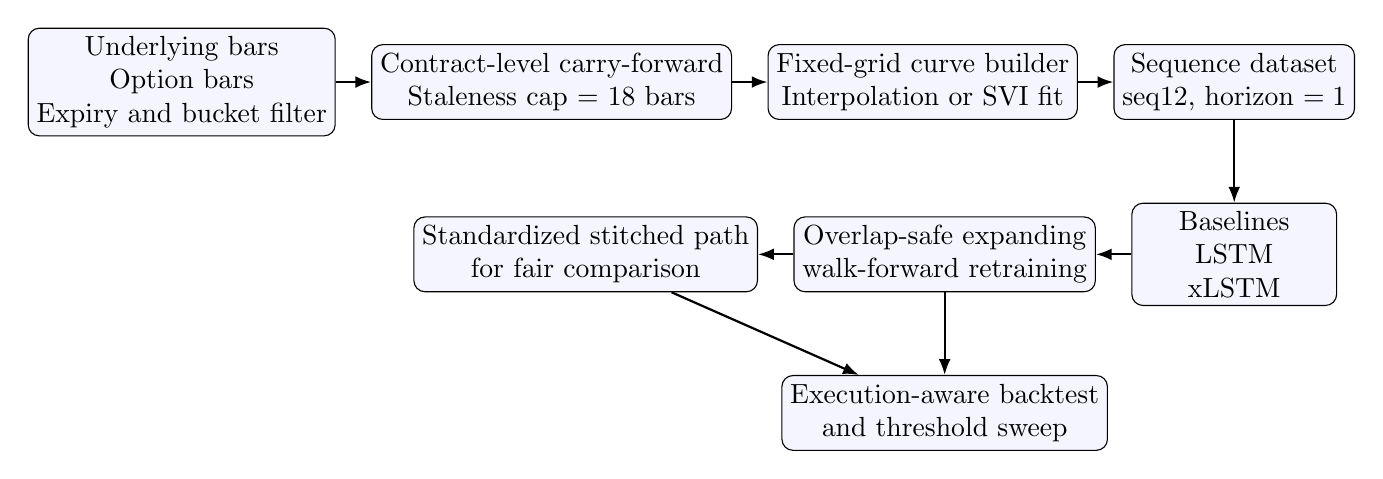
\begin{tikzpicture}[
    node distance=1.05cm and 0.45cm,
    box/.style={draw, rounded corners, align=center, minimum height=0.95cm, minimum width=2.6cm, fill=blue!4, inner sep=3pt},
    arrow/.style={-{Latex[length=2.0mm]}, thick}
]
\node[box] (raw) {Underlying bars\\Option bars\\Expiry and bucket filter};
\node[box, right=of raw] (carry) {Contract-level carry-forward\\Staleness cap = 18 bars};
\node[box, right=of carry] (curve) {Fixed-grid curve builder\\Interpolation or SVI fit};
\node[box, right=of curve] (dataset) {Sequence dataset\\seq12, horizon \(=1\)};
\node[box, below=of dataset] (models) {Baselines\\LSTM\\xLSTM};
\node[box, left=of models] (wf) {Overlap-safe expanding\\walk-forward retraining};
\node[box, left=of wf] (std) {Standardized stitched path\\for fair comparison};
\node[box, below=of wf] (bt) {Execution-aware backtest\\and threshold sweep};
\draw[arrow] (raw) -- (carry);
\draw[arrow] (carry) -- (curve);
\draw[arrow] (curve) -- (dataset);
\draw[arrow] (dataset) -- (models);
\draw[arrow] (models) -- (wf);
\draw[arrow] (wf) -- (std);
\draw[arrow] (wf) -- (bt);
\draw[arrow] (std) -- (bt);
\end{tikzpicture}%
}
\caption{Methodology pipeline for the final benchmark. The study starts from intraday market data, reconstructs a denser fixed-grid IV panel, trains each model under expanding-window retraining, and evaluates both forecasting accuracy and execution-aware trading performance on one standardized out-of-sample path.}
\label{fig:pipeline}
\end{figure}

\section{Data engineering and curve construction}
The main data-engineering challenge is not missing timestamps but cross-sectional sparsity. At many 5-minute timestamps, too few option contracts trade across moneyness to identify a stable smile slice directly. This matters because the thesis forecasts a fixed seven-node curve rather than a single scalar. If the underlying cross-section is too thin, curve quality becomes the bottleneck before modeling even begins.

The final benchmark addresses this with contract-level carry-forward. If a contract does not trade in a given 5-minute bar, its last observed option value is carried forward on the trading calendar up to a maximum staleness of 18 bars, or 90 minutes. The fill occurs at the contract level first, after which moneyness is recomputed and the fixed-grid curve is reconstructed. This is more defensible than carrying forward already-fitted grid nodes, because it preserves the link between current spot, current maturity bucket, and the contracts used to construct the smile.

The main benchmark uses this carry-forward layer together with interpolation-based curve construction. A supporting sensitivity study then replaces the interpolation layer with SVI fitting where possible. The SVI benchmark is useful because it tests whether structurally cleaner smile fitting improves the downstream ranking. As shown later, it improves the fit layer without overturning the forecasting hierarchy.

\section{Model classes and why they are included}
The benchmark is intentionally broad because weak comparator sets make neural claims difficult to interpret.

\textbf{Classical and tabular baselines.} The final library includes persistence, AR(1) per grid point, factor AR/VAR, a GARCH-style ATM-shift model, ElasticNet, MLP, ExtraTrees, histogram gradient boosting, HAR factor forecasting, and a smile-coefficient baseline. These models represent local persistence, long memory, sparse linear regularization, nonlinear tabular interactions, and curve-structure preservation. They are not included as strawmen; they are included because the literature shows that such models remain strong in volatility forecasting \citep{engle1982,bollerslev1986,corsi2009,chen2024bspline}.

\textbf{Conventional LSTM.} The LSTM family provides the baseline recurrent architecture. It is a reasonable candidate because IV curves evolve through short bursts, persistence, and local path dependence. However, the dissertation does not assume that recurrence is automatically beneficial; that is part of the empirical question.

\textbf{xLSTM.} The xLSTM family is the architectural extension tested in this study \citep{beck2024xlstm}. The motivation for including xLSTM is not novelty for its own sake. The relevant hypothesis is that a richer recurrent memory update may help separate noisy short-lived fluctuations from the smaller set of temporally coherent dislocations that matter economically. In this environment, the implemented path uses the portable \code{mLSTM}-based configuration rather than the CUDA-only \code{sLSTM} variant.

\section{Validation protocol and economic evaluation}
The final carry benchmark uses the 5-minute carry-forward dataset with 50,019 supervised samples, sequence length 12, and one-bar-ahead targets. The walk-forward split uses:
\begin{itemize}[leftmargin=1.2cm]
    \item initial train size: 17,630;
    \item validation size: 3,526;
    \item test size: 3,526;
    \item step size: 1,763;
    \item overlap-safe frontier stitching.
\end{itemize}
This produces 15 expanding-window folds without duplicated timestamps in the stitched out-of-sample path.

Two economic views are reported. The first is a fixed-threshold benchmark at \(\tau=0.0015\), which answers the question: under one common decision rule, which model is strongest? The second is a descriptive threshold sweep over
\[
\tau \in \{0.0015,0.0020,0.0025,0.0030,0.0040,0.0050,0.0075,0.0100\},
\]
which answers a different question: which models produce the most useful high-confidence signals once weak actions are filtered out? This second view matters because an options desk often cares more about the quality of a sparse actionable subset than about small average errors near zero.

\section{Robustness framing}
The dissertation includes several layers of rigor, but it is careful not to overstate what each layer proves. The completed evidence includes standardized walk-forward comparison, fixed-threshold and threshold-swept backtests, a winner-versus-all-baselines appendix pack for the final retuned xLSTM, pairwise Diebold--Mariano predictive-accuracy tests \citep{diebold1995}, and a block-bootstrap significance analysis for tuned net PnL and Sharpe on the final economic frontier. The appendix pack reports matched moneyness-region, regime-split, and execution-sensitivity comparisons against the full baseline library on the standardized retuned-carry window. The carry-plus-SVI experiment serves as a targeted data-layer sensitivity check. Together, these layers support a disciplined claim: the final xLSTM is the realized economic winner on the main carry benchmark, but it does not become the dominant statistical forecaster and it does not separate cleanly from the strongest baseline cluster on every inferential view.

\chapter{Experimental Design and Implementation}

\section{The main benchmark as the dissertation's core experiment}
The dissertation is organized around one main experiment and one supporting sensitivity check. The main experiment is the 5-minute carry-forward benchmark with one standardized out-of-sample path, the full baseline library, the retuned LSTM family, and the xLSTM extension under the same execution rules. This is the experiment from which the headline findings are drawn.

Table~\ref{tab:design_summary} summarizes the main design.

\begin{table}[H]
\centering
\caption{Main experimental design for the dissertation's primary benchmark.}
\label{tab:design_summary}
\footnotesize
\renewcommand{\arraystretch}{1.15}
\begin{tabularx}{\textwidth}{@{}lY@{}}
\toprule
\textbf{Component} & \textbf{Specification} \\
\midrule
Underlying & SPY \\
Sampling frequency & 5-minute bars \\
Target maturity bucket & 30 \(\pm\) 7 days to expiry \\
Forecast target & Seven-node fixed moneyness IV curve \\
Moneyness grid & \(-0.15,-0.10,-0.05,0.00,0.05,0.10,0.15\) \\
Supervised dataset size & 50,019 samples (carry-forward benchmark) \\
Sequence / horizon & seq12, one-bar ahead \\
Model families & 10 baselines, 4 LSTM variants, 4 xLSTM variants \\
Validation design & 15-fold expanding walk-forward, overlap-safe frontier stitching \\
Economic layer & Execution-aware backtest with exposure caps and transaction costs \\
Reporting views & Fixed threshold benchmark and descriptive threshold sweep \\
\bottomrule
\end{tabularx}
\end{table}

This design reflects the core thesis objective. It is not simply a forecasting contest. It is a benchmark built to distinguish models that minimize average error from models that produce actionable, high-conviction mispricing signals.

\section{Implementation and repository architecture}
The system is implemented as a modular pipeline with four layers:
\begin{enumerate}[leftmargin=1.2cm]
    \item data-provider and preprocessing modules for underlying bars, option bars, carry-forward, and curve fitting;
    \item dataset builders for fixed-grid supervised sequences;
    \item model modules for baselines, conventional LSTM, and xLSTM;
    \item evaluation modules for walk-forward training, standardized stitching, statistical testing, and backtesting.
\end{enumerate}

This material is kept in the experimental-design chapter rather than in the early conceptual framing because it is part of reproducibility, not problem definition. The implementation separation matters empirically: it allows the dissertation to change the data layer, such as switching from interpolation to SVI, without rewriting the downstream model-training and evaluation stack.

\section{Supporting sensitivity: carry plus SVI}
The dissertation includes one focused sensitivity study that replaces the carry-only interpolation layer with carry plus SVI smoothing. The purpose is not to rerun an entirely separate thesis, but to test whether a more structured smile-construction layer improves the downstream model ranking. This is an important distinction. The SVI study is interpreted as evidence about the \emph{data layer} rather than as the final architecture-selection benchmark, because the main retuned carry experiment remains the central comparison.

\chapter{Results and Analysis}

\section{The main finding: the statistical winner and the economic winner differ}
Table~\ref{tab:main_results} presents the core result of the dissertation. The fixed-threshold benchmark and the threshold-swept benchmark answer different questions and therefore should not be conflated. The fixed-threshold benchmark asks which model is strongest under one common decision rule. The threshold-swept benchmark asks which model becomes most economically attractive after weak signals are filtered out on the same standardized path.

\begin{table}[H]
\centering
\caption{Main retuned carry benchmark on the standardized seq12 one-bar-ahead path. The threshold-swept columns are descriptive and are computed on the same standardized prediction path.}
\label{tab:main_results}
\footnotesize
\setlength{\tabcolsep}{4pt}
\renewcommand{\arraystretch}{1.15}
\begin{tabular*}{\textwidth}{@{\extracolsep{\fill}} l l r r c r @{}}
\toprule
\textbf{Model} & \textbf{Family} & \textbf{RMSE} & \textbf{Fixed net PnL} & \textbf{Best \(\tau\)} & \textbf{Tuned net PnL} \\
\midrule
ElasticNet & Baseline & 0.010886 & 0.100416 & 0.0025 & 0.110865 \\
xLSTM b2/e256 & xLSTM & 0.013914 & -0.004776 & 0.0050 & 0.121296 \\
MLP & Baseline & 0.012646 & 0.000977 & 0.0030 & 0.115634 \\
HAR factor & Baseline & 0.013573 & 0.084505 & 0.0030 & 0.114551 \\
Smile coefficient & Baseline & 0.020815 & 0.068293 & 0.0030 & 0.109536 \\
LSTM 2x128 & LSTM & 0.033279 & -3.787900 & 0.0100 & -0.386723 \\
\bottomrule
\end{tabular*}
\vspace{0.4em}

{\footnotesize\emph{Interpretation.} ElasticNet is the statistical leader and remains near the economic frontier. xLSTM b2/e256 becomes the strongest tuned economic model after threshold filtering. The conventional LSTM family remains materially weaker on both the statistical and economic views.}
\end{table}

\insertassetfigure{Retuned carry benchmark trade-off between statistical accuracy and tuned economic value. ElasticNet remains the statistical leader on RMSE, while xLSTM b2/e256 becomes the strongest model by tuned net PnL after threshold filtering.}{fig:tradeoff}{fig_carry_retuned_tradeoff.png}

The benchmark therefore does not support a blanket statement that recurrent models dominate classical alternatives. What it supports is more precise and more interesting. ElasticNet is the best average forecaster on the standardized test path. xLSTM becomes the strongest economic model only after the signal is filtered for high-confidence actions. This is exactly the kind of divergence that a practitioner should care about: the model that best minimizes average error is not necessarily the model that produces the best monetizable edge under cost.

The rest of the frontier is also informative. MLP, HAR factor forecasting, and the smile-coefficient baseline remain close to the tuned economic frontier, which reinforces the point that this is a hard benchmark and that the baseline library is not weak. In the completed winner-versus-all-baselines appendix, the xLSTM lead is 0.0104 net PnL over ElasticNet, 0.0067 over HAR, 0.0057 over MLP, and 0.0118 over the smile-coefficient baseline on the same standardized path after each model is evaluated at its own best threshold. Those margins support xLSTM as the realized winner, but not as a runaway winner. The conventional LSTM, by contrast, is not merely slightly worse than the top models; it sits far from the frontier and fails to convert forecast variation into a selective, positive signal.

\section{Why xLSTM leads after threshold filtering}
The best xLSTM does not win by trading more often. It wins by becoming more selective. On the retuned carry benchmark, xLSTM b2/e256 is strongest at threshold \(\tau=0.0050\), not at the fixed benchmark threshold of 0.0015. Under that stricter setting it generates only 88 trades across 28,208 evaluation periods and reaches Sharpe 3.876. The best conventional LSTM still requires a much higher threshold of 0.0100 and remains negative.

\insertassetfigure{Thresholded xLSTM equity curve on the retuned carry benchmark. The plot corresponds to xLSTM b2/e256 at its best descriptive threshold \(\tau=0.0050\). The important feature is selectivity and smoothness rather than the absolute scale of cumulative PnL.}{fig:xlstm_equity}{fig_xlstm_thresholded_equity_curve.png}

Figure~\ref{fig:xlstm_equity} illustrates the practical implication. The xLSTM does not dominate the entire score distribution. Instead, it appears to rank the extreme tail of opportunities better than the conventional LSTM, and well enough to overtake the top baselines on tuned net PnL. This matters because the economic layer is vega-weighted and cost-sensitive. Once trades are thresholded, the value of a model depends less on small errors near zero and more on whether its largest predicted dislocations correspond to genuinely tradable events.

This is also the strongest conceptual reason for including xLSTM in the dissertation. A richer recurrent memory block is justified here not because it guarantees better average forecasting, but because it may better preserve regime persistence, local state shifts, and transient but economically relevant intraday structure. The evidence in this dissertation is consistent with that interpretation. It is not a mechanistic proof of what the memory block learns, but it is a coherent empirical reason why economic leadership can differ from statistical leadership.

\section{Why the conventional LSTM remains weak}
The plain LSTM problem is not merely undertraining. Its tuned net PnL stays negative and its trade profile remains too eager relative to the top models.

That pattern is informative. The dissertation is not concluding that recurrence is useless. It is showing that the form of recurrence matters. The conventional LSTM appears to convert moderate score fluctuations into too many weak trades, which is exactly the wrong behaviour once transaction costs are introduced. In contrast, the best xLSTM configuration behaves more like a sparse scoring model: fewer trades, stronger average conviction, and better conversion of forecast variation into monetizable edge.

\section{What the SVI sensitivity does and does not show}
The carry-plus-SVI sensitivity is useful because it separates structural smile fitting from downstream predictive value. Contract-level carry-forward makes SVI feasible on most slices, which means the SVI experiment is not failing merely because the smile cannot be calibrated.

\insertassetfigure{Fit-method mix in the SVI carry panel. Contract-level carry-forward makes direct SVI fitting feasible on 92.8\% of rows, so the sensitivity genuinely tests a structure-aware curve layer rather than a mostly failed calibration routine.}{fig:svi_fit_mix}{fig_svi_carry_fit_mix.png}

Figure~\ref{fig:svi_fit_mix} shows that 46,427 of 50,031 rows in the SVI panel are direct SVI fits, with only 2,760 interpolation fallbacks and 844 flat-fill cases. The data layer is therefore materially improved relative to the earlier sparse panel. Yet the downstream ranking still does not improve. In the carry benchmark, ElasticNet achieves RMSE 0.010886 and xLSTM b2/e256 achieves RMSE 0.015034. In the SVI benchmark, those values worsen to 0.015476 and 0.019468 respectively. Economically, ElasticNet remains the leader in the completed SVI family benchmark, and xLSTM remains the best neural model but falls further behind.

The right interpretation is not that SVI is mathematically wrong. It is that structurally cleaner curve fitting does not automatically create a better prediction target for this task. On this dataset, the bottleneck remains the extraction of a stable, monetizable short-horizon signal, not only the smoothness of the fitted smile.

\section{Statistical interpretation: why the forecast-loss ranking still matters}
The economic evidence should be read together with the forecast-loss evidence, not against it. Pairwise Diebold--Mariano tests \citep{diebold1995} on the carry retuned appendix pack show that xLSTM b2/e256 does \emph{not} become the dominant statistical forecaster once it is compared against every baseline on the same standardized path. ElasticNet still defeats xLSTM decisively on overall and ATM forecast loss, with DM statistic \(31.75\) overall and \(10.73\) at ATM, both with \(p=0.0\). xLSTM also loses overall to AR(1), persistence, GARCH, MLP, and HAR. Conversely, it beats ExtraTrees, smile-coefficient forecasting, and factor AR/VAR on overall loss, and it outperforms MLP, ExtraTrees, histogram gradient boosting, factor AR/VAR, and the smile-coefficient baseline on the ATM node. In the carry-plus-SVI family comparison, the same basic pattern remains: ElasticNet stays ahead statistically, with overall DM statistic \(-24.18\) in its favor against xLSTM and \(p=0.0\).

This distinction is the substantive finding of the dissertation. Once transaction costs, thresholding, and exposure limits are introduced, not all forecast errors matter equally. Small errors around zero are often economically irrelevant. A model can lose on average squared error yet still win economically if it places the most extreme predicted dislocations in the right places. The dissertation's benchmark is designed precisely to reveal that possibility.

The same appendix pack also sharpens how that result should be read. The xLSTM advantage is not broad-based statistical domination across regions or regimes. It remains weaker than ElasticNet in both high-ATM-IV and low-ATM-IV regimes on forecast RMSE. Against some nonlinear baselines, however, the pattern is more mixed: xLSTM improves on histogram gradient boosting in the low-ATM-IV regime and on several baselines around ATM, while remaining weaker on other regions such as the put wing. That is exactly the profile one would expect from a model whose strength lies in ranking a useful subset of dislocations rather than minimizing average error everywhere.

A block-bootstrap significance check strengthens the economic interpretation while also making the remaining uncertainty explicit. Using 1,000 circular block-bootstrap replications with one-trading-day blocks, xLSTM b2/e256 retains a 95\% confidence interval of \([0.0703, 0.1710]\) for tuned net PnL and \([2.8983, 4.6860]\) for Sharpe, with bootstrap probability 1.0 of positive net PnL and positive Sharpe. This is strong evidence that the xLSTM signal is genuinely positive on the observed path rather than an artifact of a single favorable run.

\insertassetfigure{Block-bootstrap confidence intervals for tuned net PnL on the final retuned carry frontier. xLSTM b2/e256 is robustly positive, but the top baseline cluster remains close and also retains positive intervals.}{fig:bootstrap_pnl}{fig_bootstrap_net_pnl_ci.png}

The bootstrap also clarifies the competitive structure of the frontier. The xLSTM lead over histogram gradient boosting and ExtraTrees remains clearly positive under resampling, but the lead over ElasticNet, HAR, MLP, and the smile-coefficient baseline is much tighter. The 95\% net-PnL delta intervals versus ElasticNet \([{-}0.0087, 0.0327]\), HAR \([{-}0.0119, 0.0272]\), MLP \([{-}0.0196, 0.0365]\), and smile coefficient \([{-}0.0074, 0.0331]\) all cross zero, even though the realized xLSTM point estimate stays ahead in each case.

\insertassetfigure{Block-bootstrap confidence intervals for the xLSTM net-PnL lead over the strongest challengers. The figure shows that the realized economic win is positive, but its margin over the top baseline cluster is narrow rather than statistically cleanly separated.}{fig:bootstrap_delta}{fig_bootstrap_winner_delta_ci.png}

That is the right way to read the final evidence. xLSTM is the realized economic winner on the main carry benchmark, and its own positive performance is well supported by the bootstrap. At the same time, the economic frontier with ElasticNet, HAR, MLP, and the smile-coefficient baseline remains tight. This keeps the dissertation's claim disciplined: xLSTM is the strongest tuned economic model in the completed benchmark, but the result is best understood as leadership within a competitive frontier rather than decisive universal dominance.

\chapter{Discussion, Limitations, and Future Work}

\section{Implications for intraday options signal extraction}
The main implication of the dissertation is that option desks and ML researchers should not treat point forecasting and tradable signal extraction as identical tasks. A desk cares about confidence, execution feasibility, and stable monetizable edge, not only average loss. The benchmark here makes that explicit. ElasticNet is the best statistical model on the main test path, yet xLSTM becomes the best economic model after the decision layer is filtered. That is not a contradiction. It is exactly what one should expect when the objective is to trade only the strongest dislocations.

This matters operationally. A desk may rationally prefer a model that produces fewer, more stable, higher-conviction signals over one that is incrementally better on average RMSE but noisier near the trading threshold. In a cost-sensitive environment, lower-variance signal extraction can be more useful than globally lower error. The dissertation therefore argues for a broader definition of model quality in intraday options work.

\section{Limits of the current evidence}
The dissertation also has clear limits.
\begin{enumerate}[leftmargin=1.3cm]
    \item The main retuned carry benchmark is single-seed. The block bootstrap addresses uncertainty in the realized return path, but it does not replace a matched multi-seed analysis of initialization variance.
    \item The threshold sweep is descriptive on the evaluation path itself. It demonstrates calibratability, but it is not equivalent to a fully separated production threshold-selection procedure.
    \item The economic layer is execution-aware but still stylized. It is not a contract-level order-book simulator and it does not hold options to expiry.
    \item The study uses one underlying and one maturity bucket, so its external validity is naturally narrower than that of a broader cross-underlying benchmark.
    \item The SVI evidence is best interpreted as a curve-construction sensitivity rather than as a final matched neural retune. It is informative about the data layer, but it does not supersede the main carry benchmark.
\end{enumerate}

\section{Future extensions}
The most natural extensions follow directly from these limits. The first is a matched multi-seed rerun of the retuned carry benchmark. The second is a richer decomposition of where the economic advantage appears, especially across moneyness regions, market regimes, and time of day. The third is a matched placebo-and-ablation suite on the final retuned carry winner so that the role of carry-forward, thresholding, and execution frictions can be isolated under the exact same benchmark. The fourth is a more structure-aware target, such as coefficient or parameter forecasting, so that structural smile information is not used only in preprocessing. The fifth is broader validation across additional liquid underlyings and maturity buckets.

\section*{Concluding remarks}
This dissertation set out to study intraday implied-volatility curve forecasting as a trading-relevant forecasting problem rather than as a generic machine-learning benchmark. The main finding is deliberately disciplined. Strong baselines, especially ElasticNet, remain the statistical benchmark. A modern recurrent model, xLSTM b2/e256, becomes the strongest economic model on the main carry benchmark only after high-confidence filtering. The conventional LSTM family remains materially weaker. The completed appendix and bootstrap evidence sharpen that conclusion further: the xLSTM signal itself is robustly positive, but its advantage over the strongest baseline cluster is narrow rather than overwhelming. The substantive lesson is therefore not that one model class dominates everything else. It is that statistical accuracy and economic usefulness diverge in a meaningful way on this problem, and that a unified leakage-aware, execution-aware benchmark is necessary to expose that divergence. That is the dissertation's primary contribution.

\cleardoublepage
\addcontentsline{toc}{chapter}{References}
\begin{thebibliography}{99}

\bibitem{black1973}
Black, F. and Scholes, M. (1973).
\newblock The pricing of options and corporate liabilities.
\newblock \emph{Journal of Political Economy}, 81(3), 637--654.

\bibitem{dumas1998}
Dumas, B., Fleming, J., and Whaley, R.~E. (1998).
\newblock Implied volatility functions: Empirical tests.
\newblock \emph{The Journal of Finance}, 53(6), 2059--2106.

\bibitem{gu2020}
Gu, S., Kelly, B., and Xiu, D. (2020).
\newblock Empirical asset pricing via machine learning.
\newblock \emph{The Review of Financial Studies}, 33(5), 2223--2273.

\bibitem{heaton2017}
Heaton, J.~B., Polson, N.~G., and Witte, J.~H. (2017).
\newblock Deep learning in finance.
\newblock arXiv preprint arXiv:1602.06561.

\bibitem{arratia2025}
Arratia, A., El Daou, M., Kagerhuber, J., and Smolyarova, Y. (2025).
\newblock Examining challenges in implied volatility forecasting: A critical review of data leakage and feature engineering combined with high-complexity models.
\newblock \emph{Computational Economics}.

\bibitem{beck2024xlstm}
Beck, M., P\"oppel, K., Spanring, M., Auer, A., Prudnikova, O., Kopp, M., Klambauer, G., Brandstetter, J., and Hochreiter, S. (2024).
\newblock xLSTM: Extended Long Short-Term Memory.
\newblock arXiv preprint arXiv:2405.04517.

\bibitem{bernales2014}
Bernales, A. and Guidolin, M. (2014).
\newblock Can we forecast the implied volatility surface dynamics of equity options? Predictability and economic value tests.
\newblock \emph{Journal of Banking \& Finance}, 46, 326--342.

\bibitem{bollerslev1986}
Bollerslev, T. (1986).
\newblock Generalized autoregressive conditional heteroskedasticity.
\newblock \emph{Journal of Econometrics}, 31(3), 307--327.

\bibitem{borochin2025}
Borochin, P. and Zhao, Y. (2025).
\newblock The economic value of equity implied volatility forecasting with machine learning.
\newblock \emph{Journal of Empirical Finance}, 82.

\bibitem{chen2024bspline}
Chen, Z., Li, Y., and Yu, C.~L. (2024).
\newblock Modeling implied volatility surface using B-splines with time-dependent coefficients predicted by tree-based machine learning methods.
\newblock \emph{Mathematics}, 12(7), 1100.

\bibitem{cont2002dynamics}
Cont, R. and da Fonseca, J. (2002).
\newblock Dynamics of implied volatility surfaces.
\newblock \emph{Quantitative Finance}, 2(1), 45--60.

\bibitem{corsi2009}
Corsi, F. (2009).
\newblock A simple approximate long-memory model of realized volatility.
\newblock \emph{Journal of Financial Econometrics}, 7(2), 174--196.

\bibitem{diebold1995}
Diebold, F.~X. and Mariano, R.~S. (1995).
\newblock Comparing predictive accuracy.
\newblock \emph{Journal of Business \& Economic Statistics}, 13(3), 253--263.

\bibitem{engle1982}
Engle, R.~F. (1982).
\newblock Autoregressive conditional heteroskedasticity with estimates of the variance of the United Kingdom inflation.
\newblock \emph{Econometrica}, 50(4), 987--1007.

\bibitem{fischer2018}
Fischer, T. and Krauss, C. (2018).
\newblock Deep learning with long short-term memory networks for financial market predictions.
\newblock \emph{European Journal of Operational Research}, 270(2), 654--669.

\bibitem{gatheral2014arbitrage}
Gatheral, J. and Jacquier, A. (2014).
\newblock Arbitrage-free SVI volatility surfaces.
\newblock \emph{Quantitative Finance}, 14(1), 59--71.

\bibitem{hochreiter1997}
Hochreiter, S. and Schmidhuber, J. (1997).
\newblock Long short-term memory.
\newblock \emph{Neural Computation}, 9(8), 1735--1780.

\bibitem{hull2019framing}
Hull, J., Qiao, Y., and others (2019).
\newblock Machine learning in business: implied volatility and option-related prediction settings.
\newblock Referenced as part of the project literature framing.

\bibitem{hutchinson1994}
Hutchinson, J.~M., Lo, A.~W., and Poggio, T. (1994).
\newblock A nonparametric approach to pricing and hedging derivative securities via learning networks.
\newblock \emph{The Journal of Finance}, 49(3), 851--889.

\bibitem{kearney2019}
Kearney, F., Shang, H.~L., and Sheenan, L. (2019).
\newblock Implied volatility surface predictability: The case of commodity markets.
\newblock \emph{Journal of Banking \& Finance}, 108, 105657.

\bibitem{sullivan2019lstm}
Sullivan, R. (2019).
\newblock LSTM-based financial forecasting course-project style literature referenced in the project framing.
\newblock Referenced in the CA-stage literature review.

\bibitem{zhao2024garchlstm}
Zhao, X., Wang, Y., and coauthors (2024).
\newblock GARCH-LSTM style volatility modeling and neural volatility priors.
\newblock Referenced in the project literature framing.

\end{thebibliography}

\appendix

\chapter{Dataset Schema and Feature Families}
The main benchmark forecasts a seven-node IV curve in a single maturity bucket centred around 30 days to expiry. The final supervised object is therefore a sequence of multivariate feature vectors paired with the next 5-minute curve.

\begin{table}[H]
\centering
\caption{Feature families used in the main seq12 one-bar-ahead benchmark.}
\footnotesize
\renewcommand{\arraystretch}{1.15}
\begin{tabularx}{\textwidth}{@{}lY@{}}
\toprule
\textbf{Feature family} & \textbf{Role in the benchmark} \\
\midrule
Current IV grid nodes & Preserve the full fixed-moneyness curve state at time \(t\). \\
ATM and level summaries & Capture broad curve level and local anchor points. \\
Returns and spot shocks & Encode contemporaneous underlying movement linked to smile adjustment. \\
Realized-volatility features & Add short-horizon volatility-state information beyond current IV. \\
Curve-shape summaries & Provide level, slope, and curvature information in compact form. \\
Trading-activity proxies & Capture local market-state changes that may affect quote adjustment. \\
DTE / bucket information & Keep the single-bucket construction explicit and reproducible. \\
\bottomrule
\end{tabularx}
\end{table}

The carry-forward benchmark contains 50,019 supervised samples. The fixed moneyness grid is
\[
\{-0.15,-0.10,-0.05,0.00,0.05,0.10,0.15\}.
\]
The carry-plus-SVI sensitivity uses the same target geometry so that the downstream comparison remains meaningful.

\chapter{Main Benchmark Configuration and Hyperparameters}

\section{Walk-forward split}
\begin{table}[H]
\centering
\caption{Walk-forward design for the main carry benchmark.}
\footnotesize
\renewcommand{\arraystretch}{1.15}
\begin{tabularx}{\textwidth}{@{}lY@{}}
\toprule
\textbf{Setting} & \textbf{Value} \\
\midrule
Initial train size & 17,630 \\
Validation size & 3,526 \\
Test size & 3,526 \\
Step size & 1,763 \\
Fold count & 15 \\
Stitch mode & Overlap-safe frontier stitching \\
\bottomrule
\end{tabularx}
\end{table}

\section{Neural shortlist used in the retuned carry benchmark}
\begin{table}[H]
\centering
\caption{Retuned neural variants compared in the main carry experiment.}
\footnotesize
\renewcommand{\arraystretch}{1.15}
\begin{tabularx}{\textwidth}{@{}lY@{}}
\toprule
\textbf{Family} & \textbf{Variants} \\
\midrule
LSTM & 2x128, 2x256, 3x128, 3x256 \\
xLSTM & b1/e128, b2/e128, b2/e256, b3/e128 \\
\bottomrule
\end{tabularx}
\end{table}

\section{Key training and execution settings}
\begin{table}[H]
\centering
\caption{Main training and backtest settings used in the retuned carry benchmark.}
\footnotesize
\renewcommand{\arraystretch}{1.15}
\begin{tabularx}{\textwidth}{@{}lY@{}}
\toprule
\textbf{Component} & \textbf{Setting} \\
\midrule
Lookback / horizon & seq12, one-bar ahead \\
Batch size & 64 \\
Maximum epochs & 40 \\
Learning rate & 0.001 \\
Early stopping patience & 8 \\
Loss & Huber loss with neural regularization hooks \\
Per-trade exposure & 0.25 \\
Minimum trade exposure & 0.05 \\
Maximum concurrent positions & 8 \\
Gross exposure cap & 2.0 \\
Net exposure cap & 1.0 \\
Effective round-trip friction & 17 bps \\
\bottomrule
\end{tabularx}
\end{table}

\chapter{Robustness Notes}
The dissertation's main conclusions rely on a completed stack of robustness layers attached to the final retuned carry benchmark and its supporting data-layer sensitivity.

\section{Completed robustness layers}
\begin{itemize}[leftmargin=1.2cm]
    \item standardized overlap-safe walk-forward comparison;
    \item fixed-threshold economic comparison;
    \item descriptive threshold sweep on the standardized path;
    \item winner-versus-all-baselines appendix pack for the final xLSTM economic winner;
    \item pairwise Diebold--Mariano predictive-accuracy tests;
    \item block-bootstrap uncertainty analysis for tuned net PnL and Sharpe;
    \item matched regime-split and execution-sensitivity comparisons in the final appendix pack;
    \item carry-plus-SVI data-layer sensitivity.
\end{itemize}

Together, these robustness layers support the central claim of the dissertation: statistical forecast leadership and economic signal leadership diverge on this problem, and that divergence survives multiple evaluation views rather than depending on a single metric table.

\end{document}
